\documentclass{article}
\usepackage{tikz}

\begin{document}

    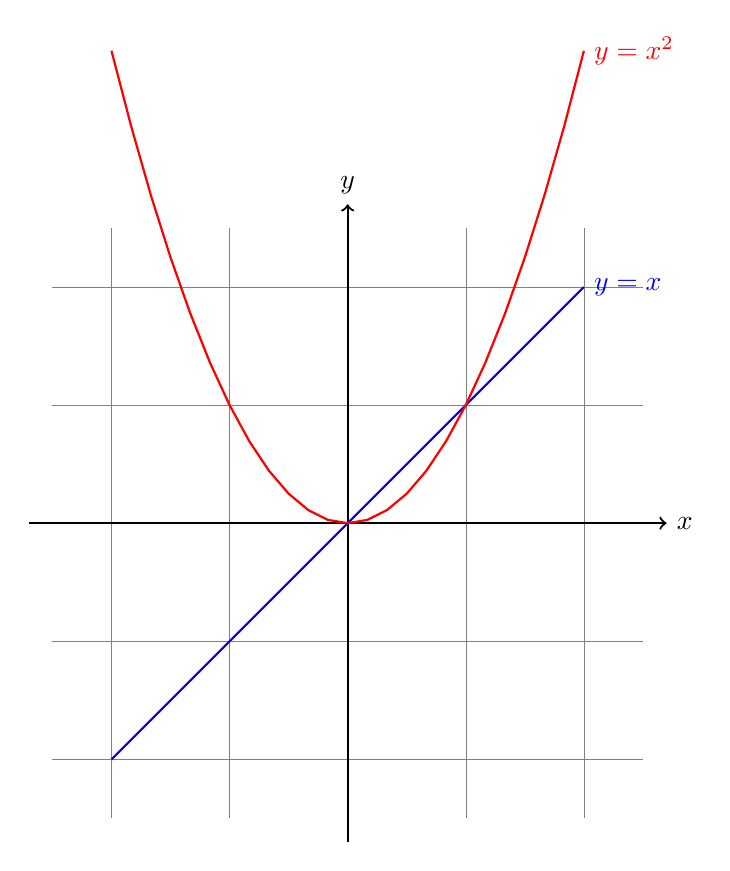
\begin{tikzpicture}[scale=1.5]
        % Draw grid
        \draw[very thin, gray] (-2.5,-2.5) grid (2.5,2.5);
        % Draw axes
        \draw[thick, ->] (-2.7,0) -- (2.7,0) node[right] {$x$};
        \draw[thick, ->] (0,-2.7) -- (0,2.7) node[above] {$y$};
        % Draw y=x and y=x^2
        \draw[blue, domain=-2:2, thick] plot (\x, \x) node[right] {$y=x$};
        \draw[red, domain=-2:2, thick] plot (\x, \x*\x) node[right] {$y=x^2$};
    \end{tikzpicture}

\end{document}
